% ---------------------------------------------------------------
% Generated by FlowTikZ (flowcharts and data charts to LaTeX)
% Every coordinate below is derived from the editor diagram model.
% Safe to edit by hand, but regenerating will overwrite changes.
% ---------------------------------------------------------------

\documentclass[border=8pt]{standalone}
\usepackage[T1]{fontenc}
\usepackage[utf8]{inputenc}
\usepackage{amsmath}
\usepackage{amssymb}
\usepackage{xcolor}
\usepackage{tikz}
\usepackage{cancel}

% ---- Colour definitions ----
\definecolor{fc12161C}{HTML}{12161C}
\definecolor{fcD97706}{HTML}{D97706}
\definecolor{fcDC2626}{HTML}{DC2626}
\definecolor{fcFEF3C7}{HTML}{FEF3C7}

% ---- Style definitions ----
\tikzset{
  fcnode/.style={
    draw, inner sep=0pt, outer sep=0pt, align=center,
    line join=round, line cap=butt
  },
  fcpath/.style={line join=round, line cap=butt},
  fcedge/.style={line join=round, line cap=butt},
  fclabel/.style={inner sep=1.4pt, outer sep=0pt, align=center},
}
\tikzset{fcformula/.style={inner sep=0pt, outer sep=0pt}}

\begin{document}
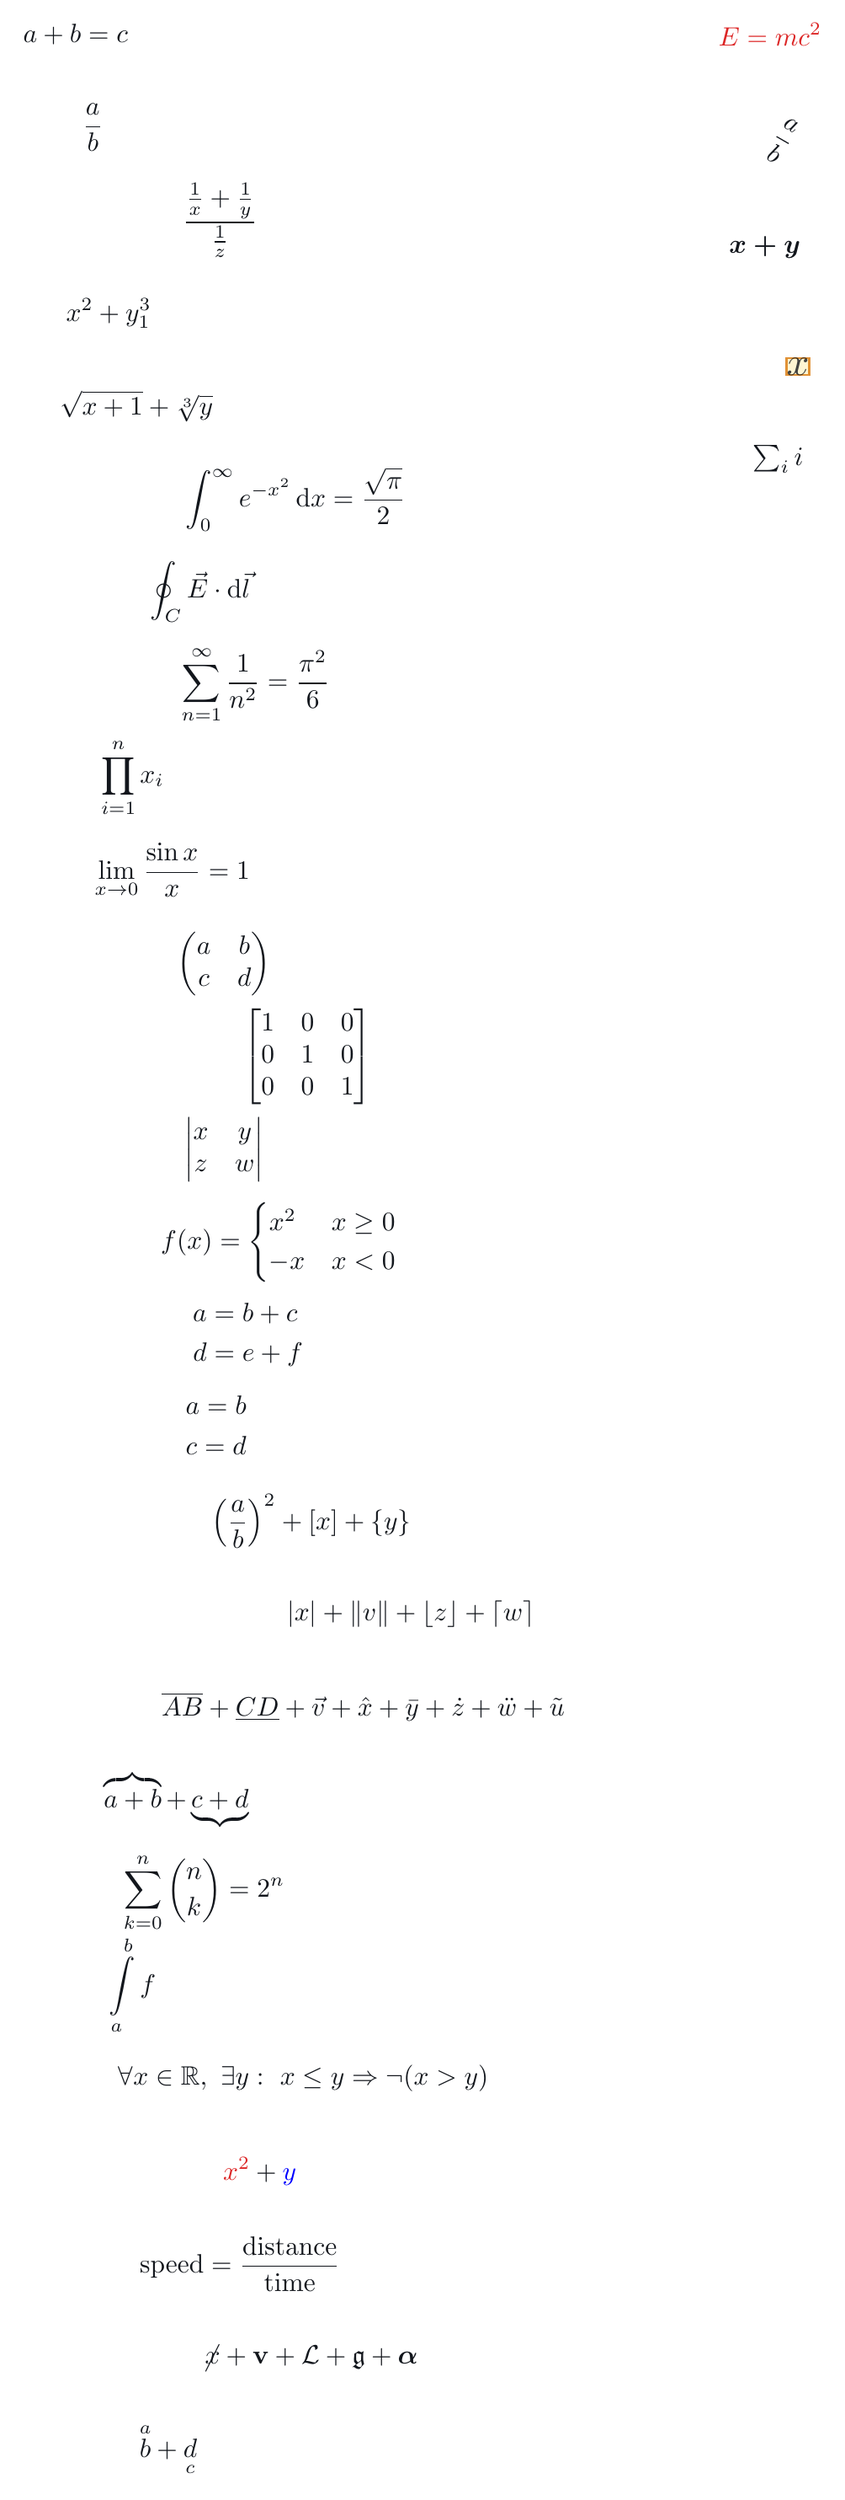
\begin{tikzpicture}[x=1cm, y=1cm]
  % ---- Nodes ----
  % n1 - Formula "a+b=c"
  \node[fcformula, scale=1.138, text=fc12161C] (n1) at (2.4,-2.4) {$\displaystyle a+b=c$};
  % n2 - Formula "\frac{a}{b}"
  \node[fcformula, scale=1.138, text=fc12161C]
        (n2) at (2.66,-3.8) {$\displaystyle \frac{a}{b}$};
  % n3 - Formula "\frac{\frac{1}{x}+\frac{1}{y}}{\frac{1}{z}}"
  \node[fcformula, scale=1.138, text=fc12161C]
        (n3) at (4.58,-5.2) {$\displaystyle \frac{\frac{1}{x}+\frac{1}{y}}{\frac{1}{z}}$};
  % n4 - Formula "x^{2}+y_{1}^{3}"
  \node[fcformula, scale=1.138, text=fc12161C]
        (n4) at (2.9,-6.6) {$\displaystyle x^{2}+y_{1}^{3}$};
  % n5 - Formula "\sqrt{x+1}+\sqrt[3]{y}"
  \node[fcformula, scale=1.138, text=fc12161C]
        (n5) at (3.32,-8) {$\displaystyle \sqrt{x+1}+\sqrt[3]{y}$};
  % n6 - Formula "\int_{0}^{\infty} e^{-x^{2}}\,\mathrm{d}x=\frac{"
  \node[fcformula, scale=1.138, text=fc12161C]
        (n6) at (5.72,-9.4) {$\displaystyle \int_{0}^{\infty} e^{-x^{2}}\,\mathrm{d}x=\frac{\sqrt{\pi}}{2}$};
  % n7 - Formula "\oint_{C}\vec{E}\cdot\mathrm{d}\vec{l}"
  \node[fcformula, scale=1.138, text=fc12161C]
        (n7) at (4.28,-10.8) {$\displaystyle \oint_{C}\vec{E}\cdot\mathrm{d}\vec{l}$};
  % n8 - Formula "\sum_{n=1}^{\infty}\frac{1}{n^{2}}=\frac{\pi^{2}"
  \node[fcformula, scale=1.138, text=fc12161C]
        (n8) at (5.12,-12.2) {$\displaystyle \sum_{n=1}^{\infty}\frac{1}{n^{2}}=\frac{\pi^{2}}{6}$};
  % n9 - Formula "\prod_{i=1}^{n} x_{i}"
  \node[fcformula, scale=1.138, text=fc12161C]
        (n9) at (3.26,-13.6) {$\displaystyle \prod_{i=1}^{n} x_{i}$};
  % n10 - Formula "\lim_{x\to 0}\frac{\sin x}{x}=1"
  \node[fcformula, scale=1.138, text=fc12161C]
        (n10) at (3.86,-15) {$\displaystyle \lim_{x\to 0}\frac{\sin x}{x}=1$};
  % n11 - Formula "\begin{pmatrix} a & b \\ c & d \end{pmatrix}"
  \node[fcformula, scale=1.138, text=fc12161C]
        (n11) at (4.64,-16.4) {$\displaystyle \begin{pmatrix} a & b \\ c & d \end{pmatrix}$};
  % n12 - Formula "\begin{bmatrix} 1 & 0 & 0 \\ 0 & 1 & 0 \\ 0 & 0 "
  \node[fcformula, scale=1.138, text=fc12161C]
        (n12) at (5.9,-17.8) {$\displaystyle \begin{bmatrix} 1 & 0 & 0 \\ 0 & 1 & 0 \\ 0 & 0 & 1 \end{bmatrix}$};
  % n13 - Formula "\begin{vmatrix} x & y \\ z & w \end{vmatrix}"
  \node[fcformula, scale=1.138, text=fc12161C]
        (n13) at (4.64,-19.2) {$\displaystyle \begin{vmatrix} x & y \\ z & w \end{vmatrix}$};
  % n14 - Formula "f(x)=\begin{cases} x^{2} & x\geq 0 \\ -x & x<0 \"
  \node[fcformula, scale=1.138, text=fc12161C]
        (n14) at (5.48,-20.6) {$\displaystyle f(x)=\begin{cases} x^{2} & x\geq 0 \\ -x & x<0 \end{cases}$};
  % n15 - Formula "\begin{aligned} a &= b+c \\ d &= e+f \end{aligne"
  \node[fcformula, scale=1.138, text=fc12161C]
        (n15) at (5,-22) {$\displaystyle \begin{aligned} a &= b+c \\ d &= e+f \end{aligned}$};
  % n16 - Formula "\begin{gathered} a=b \\ c=d \end{gathered}"
  \node[fcformula, scale=1.138, text=fc12161C]
        (n16) at (4.52,-23.4) {$\displaystyle \begin{gathered} a=b \\ c=d \end{gathered}$};
  % n17 - Formula "\left( \frac{a}{b} \right)^{2}+\left[ x \right]+"
  \node[fcformula, scale=1.138, text=fc12161C]
        (n17) at (5.96,-24.8) {$\displaystyle \left( \frac{a}{b} \right)^{2}+\left[ x \right]+\left\{ y \right\}$};
  % n18 - Formula "\left| x \right|+\left\| v \right\|+\left\lfloor"
  \node[fcformula, scale=1.138, text=fc12161C]
        (n18) at (7.46,-26.2) {$\displaystyle \left| x \right|+\left\| v \right\|+\left\lfloor z \right\rfloor+\left\lceil w \right\rceil$};
  % n19 - Formula "\overline{AB}+\underline{CD}+\vec{v}+\hat{x}+\ba"
  \node[fcformula, scale=1.138, text=fc12161C]
        (n19) at (6.74,-27.6) {$\displaystyle \overline{AB}+\underline{CD}+\vec{v}+\hat{x}+\bar{y}+\dot{z}+\ddot{w}+\tilde{u}$};
  % n20 - Formula "\overbrace{a+b}+\underbrace{c+d}"
  \node[fcformula, scale=1.138, text=fc12161C]
        (n20) at (3.92,-29) {$\displaystyle \overbrace{a+b}+\underbrace{c+d}$};
  % n21 - Formula "\sum\limits_{k=0}^{n}\binom{n}{k}=2^{n}"
  \node[fcformula, scale=1.138, text=fc12161C]
        (n21) at (4.34,-30.4) {$\displaystyle \sum\limits_{k=0}^{n}\binom{n}{k}=2^{n}$};
  % n22 - Formula "\int\limits_{a}^{b} f"
  \node[fcformula, scale=1.138, text=fc12161C]
        (n22) at (3.26,-31.8) {$\displaystyle \int\limits_{a}^{b} f$};
  % n23 - Formula "\forall x\in\mathbb{R},\ \exists y:\ x\leq y\Rig"
  \node[fcformula, scale=1.138, text=fc12161C]
        (n23) at (5.84,-33.2) {$\displaystyle \forall x\in\mathbb{R},\ \exists y:\ x\leq y\Rightarrow\neg(x>y)$};
  % n24 - Formula "\textcolor[RGB]{220,38,38}{x^{2}}+\textcolor{blu"
  \node[fcformula, scale=1.138, text=fc12161C]
        (n24) at (5.18,-34.6) {$\displaystyle \textcolor[RGB]{220,38,38}{x^{2}}+\textcolor{blue}{y}$};
  % n25 - Formula "\text{speed}=\frac{\text{distance}}{\text{time}}"
  \node[fcformula, scale=1.138, text=fc12161C]
        (n25) at (4.88,-36) {$\displaystyle \text{speed}=\frac{\text{distance}}{\text{time}}$};
  % n26 - Formula "\cancel{x}+\mathbf{v}+\mathcal{L}+\mathfrak{g}+\"
  \node[fcformula, scale=1.138, text=fc12161C]
        (n26) at (5.96,-37.4) {$\displaystyle \cancel{x}+\mathbf{v}+\mathcal{L}+\mathfrak{g}+\boldsymbol{\alpha}$};
  % n27 - Formula "\overset{a}{b}+\underset{c}{d}"
  \node[fcformula, scale=1.138, text=fc12161C]
        (n27) at (3.8,-38.8) {$\displaystyle \overset{a}{b}+\underset{c}{d}$};
  % n28 - Formula "E=mc^{2}"
  \node[fcformula, scale=1.138, text=fcDC2626]
        (n28) at (12.88,-2.4) {$\displaystyle E=mc^{2}$};
  % n29 - Formula "\frac{a}{b}"
  \node[fcformula, scale=1.138, text=fc12161C, rotate=-30]
        (n29) at (13.06,-4) {$\displaystyle \frac{a}{b}$};
  % n30 - Formula "x+y"
  \node[fcformula, scale=1.138, text=fc12161C]
        (n30) at (12.8,-5.6) {$\displaystyle \boldsymbol{x+y}$};
  % n31 - Formula "x"
  \node[fcformula, scale=1.707, text=fc12161C, draw=fcD97706, line width=0.91pt, fill=fcFEF3C7,
        fill opacity=0.7, opacity=0.8] (n31) at (13.3,-7.4) {$\displaystyle x$};
  % n32 - Formula "\sum_{i} i"
  \node[fcformula, scale=1.138, text=fc12161C] (n32) at (13,-8.8) {$\sum_{i} i$};
\end{tikzpicture}
\end{document}